\documentclass{article}
\usepackage{float}

% Basic packages
\usepackage[utf8]{inputenc}
\usepackage[T1]{fontenc}
\usepackage{lmodern}
\usepackage[margin=2.5cm]{geometry}
\usepackage{amsmath,amssymb}
\usepackage{hyperref}
\usepackage{graphicx}
\usepackage{booktabs}
\usepackage{enumitem}
\usepackage{xcolor}
\usepackage{float}
\usepackage{doi}
\usepackage{url}
\usepackage[font=small,labelfont=bf]{caption}
\captionsetup[table]{labelsep=quad}
\usepackage{ragged2e}
\usepackage{array}
\newcolumntype{L}[1]{>{\RaggedRight\arraybackslash}p{#1}}
\usepackage{enumitem}
\setlist[itemize,1]{label=---}
% Define PDL macro
\newcommand{\PDL}{\mathrm{PDL}}
\usepackage{tikz}
\usetikzlibrary{positioning}
\usepackage{longtable}
\usepackage{booktabs} % tu l'as déjà, gardons-le

\hypersetup{
  colorlinks=true,
  linkcolor=blue,
  citecolor=blue,
  urlcolor=blue
}

\title{Projective Dynamic Logo (PDL)\\
Global Mapping of Structures, Results, and Open Problems}
\author{C. Laubscher}
\date{\today}

\begin{document}

\setcounter{tocdepth}{1}

\maketitle

\begin{abstract}
This document provides a comprehensive global exposition of the Projective Dynamic Logo (PDL) framework. It organizes the extant literature into a unified and coherently structured architecture, explicates the logical interdependencies among axioms, constructions, and their corresponding physical interpretations, and classifies the resulting statements according to their epistemic status. In particular, it differentiates rigorously proven structural theorems from tightly constrained conjectural claims and from components whose parameters are determined through empirical calibration.\end{abstract}
\tableofcontents

\section{Purpose and Scope}
\label{sec:purpose_scope}

\subsection{Aim of this mapping}
\label{subsec:aim}

The purpose of this mapping document is to furnish a systematic and comprehensive overview of the Projective Dynamic Logo (PDL) programme. Rather than advancing novel technical results, it synthesises and organises the extant body of work into a coherent framework, thereby clarifying the interrelations between axioms, constructions, and physical interpretations, as well as their respective epistemic status \cite{PDL_position,PDL_intro}. More specifically, this document pursues four principal objectives: (i) to render explicit the logical dependencies among the core components of PDL (relational axioms, minimal $4$--$6$ block, proton architecture, constants, dynamics, leakage mechanisms, and emergent metric structure); (ii) to classify existing results into rigorously established structural theorems, tightly constrained conjectures, and empirically calibrated elements; (iii) to serve as a navigational instrument for the PDL corpus by means of concise summaries and systematic cross-references; and (iv) to delineate a roadmap of open problems and prospective avenues for future research \cite{PDL_position}.

\subsection{Position within the PDL corpus}
\label{subsec:position_corpus}

Within the broader PDL corpus, the present mapping is to be regarded as a meta-level document. The principal PDL/LDP article (D1) develops the complete axiomatic framework, including the derivation of the $4$–$6$ structure, the proton architecture, and the re-interpretation of several physical constants, and additionally provides an initial treatment of gravitation and cosmology \cite{PDL_Main_2026}. The introductory note (D2) presents a high-level conceptual overview accompanied by a concise summary of the principal structures and numerical correspondences \cite{PDL_intro}. The position paper (D3) analyses the current status of the framework, its epistemic stratification, and the outstanding open problems, with particular emphasis on its interface with the Theory of Objectivity \cite{PDL_position}. In contrast, the present mapping does not supersede any of these texts; rather, it systematises their content by providing an explicit dependency diagram, a unified classification of results, and a cross-referenced index of documents and thematic domains. 
Beyond these three core texts, several more recent manuscripts develop specific components of the programme in greater technical depth. In particular, the logical core and the necessity of the $(4,6)$ block are analysed in a dedicated study of minimal stationary closures \cite{Minimal_Stationary_Closures_2026}; the combinatorial selection and local uniqueness of the proton architecture are treated in a refined manner \cite{Proton_Local_Uniqueness_2026,Combinatorial_Proton_v2_2026}; and the leakage mechanism, together with the exponent $18$, is revisited in a more systematic way \cite{Coherence_Leakage_18_2026,Exponent_18_PDL_2026}.

\subsection{Intended audience}
\label{subsec:intended_audience}

The principal intended readership for this mapping consists of researchers in foundational physics, mathematical physics, quantum foundations, and cognate conceptual research programmes, including the Theory of Objectivity. It is directed toward readers who are proficient in abstract structural reasoning and discrete mathematical frameworks, and who seek a concise yet systematic exposition of the current claims of PDL, the manner in which its constituent elements form a coherent whole, and the locations of the most significant outstanding problems \cite{PDL_intro,PDL_TO_dialogue,PDL_position}. It is not designed as a popular-level introduction, nor as a substitute for the detailed technical derivations presented in the primary PDL manuscripts.

\section{Overview of the PDL Programme}
\label{sec:overview}

\subsection{Core question and methodological stance}
\label{subsec:core_question}

The PDL programme is structured around a single central research question: \emph{What are the minimal logical conditions under which an entity can exist in a temporally persistent manner, once all metric notions such as space, time, and energy have been suspended}? \cite{PDL_Main_2026,PDL_intro}

In contrast to approaches that presuppose a pre-given spacetime manifold, a fixed catalogue of elementary particles, or externally imposed dynamical laws, PDL adopts a more fundamental, pre-metric perspective. It posits solely that existence must appear as a reproducible distinction—a difference that can be repeatedly instantiated in a manner that is logically self-sufficient, does not depend on any unspecified background structure, and can be stably sustained without collapsing into an undifferentiated null state.
\cite{PDL_Main_2026,PDL_position}.

Within this framework, reality is represented as a network of minimal logical closures defined on finite signed graphs. Vertices correspond to informational entities, edges encode binary agreement/disagreement relations, and the dynamical evolution of configurations is determined by a coherence-optimisation principle rather than by externally prescribed field equations. Space, time, and other familiar physical quantities are not treated as primitive inputs but as potentially emergent structures, to be reconstructed from the coherence properties of these closures.
\cite{PDL_Main_2026,PDL_intro}.

From a methodological perspective, this entails a two-stage approach. In the first stage, one formulates purely relational axioms that encode the logical conditions for persistent existence—namely, minimal binary pulsation, triangular coherence, minimal completeness, and logical optimisation. In the second stage, one examines which discrete structures are \emph{necessarily} instantiated under these axioms and to what extent they can be coherently identified with known physical entities, such as the electron, the proton, and various dimensionless constants. The present mapping document is dedicated to explicating the manner in which this strategy is implemented throughout the existing PDL corpus. 
\cite{PDL_position}.

\subsection{List of main PDL documents}
\label{subsec:documents}

Table~\ref{tab:documents} provides an overview of the principal documents comprising the current PDL corpus, detailing their primary thematic focus and delineating their specific function within the overall programme framework.

\setlength{\LTpre}{18pt}
\setlength{\LTpost}{0pt}

\begin{longtable}{@{}llL{4cm}p{9.5cm}@{}}
\caption{Main PDL documents and their roles within the programme.}
\label{tab:documents}\\
\toprule
Label & Year & Document & Focus / Role \\
\midrule
\endfirsthead

\toprule
Label & Year & Document & Focus / Role \\
\midrule
\endhead

D1 & 2026 & \textit{The Emergence of Physical Reality within the Framework of the Projective Dynamic Logo (PDL)} &
Principal technical article: formulation of relational axioms on signed graphs; derivation of the minimal $(4,6)$ structural block; development of a hierarchical proton architecture; reinterpretation of $\hbar$, $\alpha$, $k_B$, and an effective gravitational coupling constant as coherence ratios; and preliminary construction of an emergent metric and cosmological framework. \cite{PDL_Main_2026} \\[0.5em]

D2 & 2026 & \textit{Introduction to the Projective Dynamic Logo (PDL)} &
High-level exposition of the PDL framework, including conceptual motivation, outline of the axiomatic system, presentation of the $(4,6)$ structure, analysis of the proton integers $(24,28,930,10087,11017)$, and a unified treatment of fundamental constants aimed at readers in quantum foundations and mathematical physics. \cite{PDL_intro} \\[0.5em]

D3 & 2026 & \textit{Projective Dynamic Logo as a Foundational Research Programme: Current Status, Open Problems, and Interface with the Theory of Objectivity} &
Position paper: synthesises the current state of the programme, delineates structurally robust results from conjectural or calibrated components, and formulates open problems (including uniqueness of the $(4,6)$ configuration, rigidity of the proton architecture, derivation of the leakage parameter, and dynamical extensions), with emphasis on the interface with the Theory of Objectivity. \cite{PDL_position,PDL_TO_dialogue} \\[0.5em]

D4 & 2026 & \textit{On the Combinatorial Selection of the Proton Architecture in PDL: Axiomatic Constraints, Integer Structures, and a Uniqueness Conjecture (v2)} &
Updated analysis of the proton structural configuration: formulation of integer-valued constraints, specification of an optimisation functional, and justification of the parameter tuple $(24,28,930,10087,11017)$ in its v2 form, together with a critical discussion of potential alternative architectural configurations. \cite{Combinatorial_Proton_v2_2026} \\[0.5em]

D5 & 2026 & \textit{A Structural Derivation of the Fine-Structure Constant from the Projective Dynamic Logo (PDL) (v2)} &
Closed-form expression for $\alpha^{-1}$ as a function of the proton–electron mass ratio, the valence content $r_{\mathrm{val}}=930$, and the golden ratio, achieving a relative accuracy of $\mathcal{O}(10^{-4})$ without continuous fit parameters; v2 incorporates refinements after the TO dialogue. \cite{Alpha_PDL_v2_2026} \\[0.5em]

D6 & 2026 & \textit{Relational Emergence of Born's Rule and a Golden-Ratio Active Surface in PDL (v2)} &
Derivation of Born's rule for spin-$\tfrac{1}{2}$ systems and of the fine-structure constant from finite active surfaces in signed graphs; refinement of the rôle of the golden ratio in the proton core–surface partition and its connection to $\alpha$; v2 incorporates structural clarifications. \cite{Born_Golden_v2_2026,Golden_Ratio_Sketch_2026} \\[0.5em]

D7 & 2026 & \textit{From Discrete Coherence Flux to Effective Fields: A Structured Programme within the PDL Framework} &
Development of discrete Gauss- and Faraday-like relations from mixed-triangle coherence fluxes in PDL, derivation of $1/r^2$ Coulomb profiles from shell-counting arguments, and outline of how Schr\"odinger-type dynamics can emerge from discrete coherence flux. \cite{Effective_Fields_PDL_2026} \\[0.5em]

D8 & 2026 & \textit{A Minimal Relational Sketch for the Emergence of the Golden Ratio in PDL} &
Conceptual sketch showing how a self-similar core–surface partition within the proton architecture leads to the selection of the golden ratio and constrains the effective active surface associated with $\alpha$ and surface coherence. \cite{Golden_Ratio_Sketch_2026} \\[0.5em]

D9 & 2026 & \textit{Hierarchical Filtering of Coherence Leakage and Justification of the Exponent 18 in PDL} &
Initial formulation of the leakage mechanism and of the exponent $18$ as the total number of hierarchical coherence filters linking proton-level leakage to macroscopic effective couplings; provides the original list of filters and qualitative arguments for their minimality. \cite{Exponent_18_PDL_2026} \\[0.5em]

D10 & 2026 & \textit{Logical Leakage as Self-Maintained Probability: A Topological Reformulation in the Projective Dynamic Logo Framework} &
Development of a coexistence topology and a coherence-cost pseudo-metric, reinterpreting logical leakage as an intrinsic probability of non-closure, and exploring correspondences with quantum probabilities, gravitation, and thermodynamics. \cite{Topological_Reformulation_PDL_2026} \\[0.5em]

D11 & 2026 & \textit{Compatibility of the Schr\"odinger Framework with the Projective Dynamic Logo (PDL) (v2)} &
Consistency assessment: implementation of the PDL-derived fine-structure constant and proton parameters into the nonrelativistic hydrogenic Schr\"odinger equation; verification of spectral concordance within stated accuracy; v2 updates the analysis and numerical checks. \cite{Schrodinger_PDL_v2_2026} \\[0.5em]

D12 & 2026 & \textit{Towards a Schr\"odinger--Type Dynamics from the Projective Dynamic Logo (PDL): A Relational Sketch Linking Coherence Cycles, Active Surfaces, and Effective Potentials (v2)} &
Investigation of how Schr\"odinger-like dynamical equations might emerge from intrinsically defined discrete graph evolution (Laplacians and flux balance) rather than being postulated; v2 refines the relational sketch and its consistency conditions. \cite{Schrodinger_Sketch_v2_2026} \\[0.5em]

D13 & 2026 & \textit{A Modal Dialogue between the Projective Dynamic Logo (PDL) and the Theory of Objectivity (TO)} &
Comparative study of PDL relational axioms and TO's Seven Absolute Truths; clarification of modal and ontological commitments of PDL and formal treatment of multi-observer perspectives and boundary conditions. \cite{PDL_TO_dialogue} \\[0.5em]

D14 & 2026 & \textit{Towards an Einstein--Dirac Unification from the Projective Dynamic Logo Framework} &
Extension of PDL towards a unified treatment of Einstein- and Dirac-type structures: association of Dirac spinors with $(4,6)$ electron closures, coupling to the emergent coherence-cost metric, and preliminary consistency checks based on hydrogenic limits and redshift-type scenarios. \cite{Einstein_Dirac_PDL_2026} \\[0.5em]

D15 & 2026 & \textit{Minimal Stationary Closures in the Projective Dynamic Logo Framework: Necessity of the (4,6) Block} &
Technical analysis of the logical core: reformulation of the four PDL axioms directly on finite signed graphs; introduction of a precise notion of minimal stationary closure; proof that no such closure exists for graphs with at most three vertices and that the complete signed graph on four vertices and six edges realises the first admissible elementary stationary closure, with minimality and quasi-uniqueness properties. \cite{Minimal_Stationary_Closures_2026} \\[0.5em]

D16 & 2026 & \textit{On the Combinatorial Selection and Local Uniqueness of the Proton Architecture in the PDL Framework} &
Refined combinatorial treatment of the proton architecture: definition of admissible proton configurations under structural and phenomenological constraints, introduction of a selection functional $S$, verification that the tuple $(24,28,930,10087,11017)$ is admissible and achieves a high selection score, and formulation of an explicit local uniqueness conjecture and search programme. \cite{Proton_Local_Uniqueness_2026,Combinatorial_Proton_v2_2026} \\[0.5em]

D17 & 2026 & \textit{Coherence Leakage, Hierarchical Filtering, and the Exponent 18 in the Projective Dynamic Logo Framework} &
Refined treatment of coherence leakage and the exponent $18$: definition of the minimal closure defect $\varepsilon$ on a class of admissible proton graphs, interpretation of $\varepsilon$ as an intrinsic coherence leakage parameter, organisation of the eighteen coherence filters into three hierarchical blocks, and formulation of an effective coupling ansatz $G_{\mathrm{eff}}^{\PDL}=C\,\varepsilon^{n}$ together with qualitative constraints. \cite{Coherence_Leakage_18_2026,Topological_Reformulation_PDL_2026,Effective_Fields_PDL_2026} \\[0.5em]

\bottomrule
\end{longtable}

\subsection*{Reading guide}

For readers approaching PDL for the first time, the following minimal reading pathways are recommended. To develop an understanding of the logical foundations of the programme — encompassing the axiomatic framework, the minimal $4$--$6$ structure, and the formal representations of the electron and proton—priority should be given to Sections~\ref{sec:logical_core}, \ref{sec:four_six_electron}, and \ref{sec:proton_architecture}. For an examination of the reinterpretation of constants as coherence ratios and the concomitant emergence of gravitation and metric structure, Sections~\ref{sec:constants} and \ref{sec:topology_metric} should be consulted. A concise overview of the present status of the theory, differentiating structurally established results from conjectural or calibrated components, is provided by the global result map in Section~\ref{sec:global_map}, and in particular by Table~\ref{tab:status}. Finally, Section~\ref{sec:roadmap} offers a synthesis of the principal open problems and delineates prospective directions for further research.

\section{Logical Core: Axioms and Minimal Structures}
\label{sec:logical_core}

\subsection{Relational axioms on signed graphs}
\label{subsec:axioms}

In PDL, a logical configuration is formalised as a finite signed graph \(G = (V, E)\), where the vertices in \(V\) represent informational entities and the edges in \(E\) are endowed with signs \(s_{ij} \in \{+1, -1\}\) that encode pairwise agreement/disagreement relations \cite{PDL_Main_2026,PDL_intro}. On this discrete structural substrate, four relational axioms are postulated:

\begin{itemize}[leftmargin=1.5em]
  \item \textbf{Minimal binary pulsation:} existence is instantiated as a repeatable alternation between two discrete states that does not presuppose any underlying temporal metric; formally, a discrete dynamical system on a space of sign configurations is required to admit at least one logical 2-cycle.

  \item \textbf{Triangular coherence:} closed cycles of length three (triangles) constitute elementary closure motifs. Each violated triangle—either through the absence of a required edge or through the failure of a coherence condition on the product of signs—incurs a penalty in a stability functional.

  \item \textbf{Minimal completeness:} elementary stationary structures must be both closed and logically autonomous: all referential dependencies necessary to sustain the constitutive distinction are required to remain internal to the structure, without recourse to any external background or environment.

  \item \textbf{Logical optimisation:} among all admissible configurations, those that are dynamically stable are selected by maximising a functional that jointly favours low violation of triangular coherence, sufficient relational connectivity, and structural minimality, under the constraint of closure.
\end{itemize}

Collectively, these axioms formalise the thesis that persistent existence is realised as a closed, self-sustaining relational pattern that minimises logical inconsistency (violated triangles) and suppresses superfluous relational redundancy, while preserving sufficient connectivity to continuously propagate the underlying constitutive distinction \cite{PDL_Main_2026,PDL_position}.

\subsection{Closures and coherence measures}
\label{subsec:closures}

Within this framework, a \emph{closure} is defined as a finite signed graph that realises a self-contained regime of coherence under the axioms stated above. For a given configuration \(G=(V,E)\) with sign assignment \(s\), the fraction of violated triangles is given by
\[
  \epsilon = \frac{\text{number of violated triangles in } G}{\binom{|V|}{3}} \, ,
\]
with the convention \(\epsilon = 0\) if \(|V| < 3\). A triangle is classified as violated if at least one of its edges is absent or if the product of the three associated signs fails to satisfy the closure condition prescribed by the triangular coherence axiom
\cite{PDL_Main_2026}.

An optimisation functional is then introduced, depending on \(\epsilon\), on a normalised measure of connectivity, and on an indicator of structural minimality. Elementary stationary structures are defined as those configurations that saturate closure (i.e., exhibit no violated triangles), are complete and connected, exhibit no internal hierarchy among vertices, and admit a binary pulsation that preserves coherence. These structures serve as minimal logical primitives or building blocks \cite{PDL_Main_2026,PDL_position}.

\subsection{Emergence of the minimal 4--6 block}
\label{subsec:4_6_block}

A systematic elimination of inadequate configurations demonstrates that no graph with fewer than four vertices can instantiate a homogeneous, non-hierarchical closure satisfying the specified axioms. For \(n = 1,2\), triangular subgraphs are entirely absent, and for \(n = 3\) a single triangle is insufficient to support the network of overlapping coherent cycles required for the propagation of internal reference. In each of these cases, the resulting structure either fails to achieve closure, violates autonomy, or induces an implicit hierarchy \cite{PDL_Main_2026}.

The simplest configuration not excluded by these constraints is the complete graph on four vertices with six edges, denoted \(4,6\). For this graph, one can construct a sign assignment such that all triangular subgraphs are coherent (\(\epsilon = 0\)), the union of coherent triangles forms a single connected block, all vertices are structurally equivalent, and a global sign inversion realises a logical 2-cycle that preserves triangular coherence
\cite{PDL_Main_2026,PDL_intro}. In this sense, the \(4,6\) configuration constitutes the first admissible elementary stationary closure and is identified as the minimal logical building block of the model.

\subsection{Epistemic status of the logical core}
\label{subsec:logical_status}

The formulation of the axioms, the construction of the coherence measure, and the identification of the \(4,6\) configuration as the first admissible elementary stationary structure are established as structurally robust results within the PDL framework. They are derived from explicit combinatorial analysis and do not depend on phenomenological assumptions. Outstanding at this stage are, first, a comprehensive uniqueness theorem demonstrating that no alternative, comparably minimal structure can satisfy the same set of conditions, and second, a more systematic investigation of neighbouring configurations that could realise variant closure regimes \cite{PDL_position}. These open problems are explicitly represented in the global result map in Section~\ref{sec:global_map}.

\section{From 4--6 to the Electron}
\label{sec:four_six_electron}

\subsection{Logical stationary regime and internal pulsation}
\label{subsec:logical_stationary}

Crossing the threshold determined by the \((4,6)\) structure does not introduce a new ontological category of entity, but rather a new \emph{dynamical regime}. Once the complete graph on four vertices endowed with a coherent sign assignment is instantiated, the internal pattern of agreement and disagreement can no longer dissipate without infringing triangular closure constraints. In this situation, the configuration exhibits an intrinsic logical 2-cycle in the space of sign assignments: a global sign inversion returns the system to its original configuration after two iterations, while preserving overall coherence
\cite{PDL_Main_2026,PDL_intro}.

This dynamical organisation is referred to as a \emph{logical stationary regime}. It is “stationary” not in the sense of dynamical inactivity, but insofar as the internal alternation is perfectly self-sustaining: the distinction that grounds the system’s existence is continuously propagated within the closed structure without the need for exogenous input. At this stage, no specific temporal metric is assumed; only the existence of a period-2 orbit in the configuration space is posited
\cite{PDL_Main_2026,PDL_position}.

\subsection{Minimal correspondence with the electron}
\label{subsec:electron_correspondence}

Within contemporary physics, the electron at rest constitutes the first empirically accessible entity that conforms to the qualitative characteristics of this logically defined stationary regime: it is strictly stable, displays no experimentally resolvable internal substructure, and possesses an intrinsic oscillatory behaviour associated with its rest mass through the Compton frequency. In the framework of PDL, the claim is not that the \(4,6\) graph \emph{is} the electron in a strong ontological sense, but rather that the electron at rest realises the first admissible elementary stationary closure selected by the axiomatic structure of the theory \cite{PDL_Main_2026,PDL_intro}.

Within this minimal correspondence, the logical 2-cycle of the \(4,6\) configuration is identified with the physical Compton oscillation of the electron. The reduced Planck constant \(\hbar\) is thereby reinterpreted as the minimal quantum of action associated with one complete cycle of this internal coherence. In this context, the familiar relation \(E = \hbar \omega\) becomes a quantitative statement of the coherence cost required to maintain the stationary regime determined by the electron mass \cite{PDL_Main_2026}.

\subsection{Energy as coherence cost}
\label{subsec:energy_coherence}

From the PDL perspective, energy is not treated as a primitive scalar quantity assigned to a pre-existing ontological substrate, but rather as a measure of the amount of coherence budget that is committed to sustaining a given stationary regime. Each internal cycle of the \(4,6\) structure carries an irreducible quantum of action \(\hbar\), and the rest energy of the electron quantifies the cost associated with the continuous re-establishment of this logical closure. Once the \(4,6\) block is stabilised, the distinction it encodes cannot be removed without inducing a contradiction in the underlying graph structure \cite{PDL_Main_2026,PDL_intro}.

Within this framework, one can consistently introduce the notion of \emph{logical localisation} of energy prior to the specification of any spatial metric. Distinct stationary regimes can be assigned different coherence costs, such that energy becomes linked to specific organisational patterns of closure rather than to points in a pre-defined background space. Proper time, as discussed in later sections, is consequently reinterpreted as a count of internal coherence cycles, instead of being treated as an externally imposed continuous parameter \cite{PDL_Main_2026,PDL_position}.

\subsection{Status and open questions}
\label{subsec:electron_status}

The construction of the \(4,6\) block and the demonstration of the existence of a logical 2-cycle are structural results obtained directly from the axioms. The identification of this regime with the electron at rest is, by contrast, a \emph{minimal physical hypothesis}: it is adopted because the electron is the first empirically known entity that realises a strictly stable, pulsating, structureless regime compatible with the \(4,6\) properties \cite{PDL_intro}.

Open problems include the possibility of establishing uniqueness theorems demonstrating that no other elementary particle can consistently occupy this role within PDL, as well as determining the extent to which relativistic corrections and spinorial structure can be reconstructed from the same combinatorial substrate. These questions are systematically monitored in the global result map in Section~\ref{sec:global_map} \cite{PDL_position}.

\section{Hierarchical Proton Architecture}
\label{sec:proton_architecture}

\subsection{Combinatorial constraints and optimisation}
\label{subsec:proton_constraints}

Beyond the elementary \(4,6\) closure, PDL models the proton as a minimally complex hierarchical composite rather than as a structureless effective degree of freedom. The same optimisation functional used to select the \(4,6\) block is applied to construct larger configurations subject to explicit constraints: multiplicity in units of four (tetrads), near-maximal triangular coherence, net charge \(+1\), and a prescribed partitioning between quasi-stationary and dynamical relations \cite{PDL_Main_2026,Combinatorial_Proton_v2_2026}.

Within this framework, the proton is represented as comprising three local valence cores, each realised as a superposition of logical tetrads, embedded in a dense relational background and terminating at a finite active surface. The selection principle is purely combinatorial: within the class of admissible architectures satisfying the constraints above, one searches for those that locally maximise coherence while remaining minimally complex \cite{Combinatorial_Proton_v2_2026,PDL_intro}.

\subsection{Integer invariants of the proton model}
\label{subsec:proton_integers}

The combinatorial analysis identifies a specific set of integer invariants characterising the proton’s internal architecture: valence occupancies \(n_u = 24\) and \(n_d = 28\), a total valence relational content \(r_{\mathrm{val}} = 930\), a dynamical sea with \(R_{\mathrm{sea}} = 10087\) relations, and an overall internal relational budget \(R_{\mathrm{tot}} = 11017\) \cite{Combinatorial_Proton_v2_2026,PDL_intro}. Taken together, these quantities imply an approximate decomposition of the proton’s internal coherence into \(\sim 9\%\) quasi-stationary and \(\sim 91\%\) dynamical contributions, which is qualitatively compatible with QCD-inspired descriptions in which the dominant fraction of the proton mass emerges from gluonic and sea-quark dynamics rather than from static valence degrees of freedom.

A key feature of this framework is that these integers are not postulated independently for distinct physical effects. Instead, they constitute a tightly constrained structural backbone that simultaneously governs internal stability, the coupling of the proton’s surface to electrons, the channels and rates of information and energy leakage, and the calibration of effective constants. The same integer tuple \((24,28,930,10087,11017)\) reappears in the proposed derivations of the fine-structure constant, in the reinterpretation of Boltzmann’s constant, and in the formulation of an effective gravitational coupling \cite{PDL_intro,Alpha_PDL_v2_2026,Born_Golden_v2_2026}.

\subsection{Active surface and relational sea}
\label{subsec:active_surface}

In the Proton Description Layer (PDL) framework, the proton’s internal hierarchical structure is organised into three distinct levels: quasi-stationary valence cores, a highly interconnected dynamical relational sea, and a finite active surface. The valence cores localise and stabilise internally saturated coherence; the relational sea mediates the dynamical redistribution and reconfiguration of these internal relations; and the active surface encodes the finite set of coupling channels through which the proton interacts both with external \(4,6\) blocks (electrons) and with the ambient relational network
\cite{PDL_Main_2026,Born_Golden_v2_2026}.

Within this framework, the active surface is central to the reinterpretation of dimensionless fundamental constants, such as the fine-structure constant \(\alpha\), in terms of ratios of internal coherence to surface coherence. It furthermore provides the natural locus for modelling the leakage of coherence from composite nucleonic configurations into their environment—an effect that, in the PDL approach, forms the basis for the emergence of an effective gravitational coupling
\cite{Alpha_PDL_v2_2026,Exponent_18_PDL_2026}.

\subsection{Epistemic status and possible alternatives}
\label{subsec:proton_status}

The qualitative, hierarchical representation of the proton as comprising three valence cores, a relational sea, and an active surface is firmly grounded in the PDL axioms and the associated optimisation strategy. The particular integer tuple \((24,28,930,10087,11017)\) is, at present, supported both by focused combinatorial searches and by its demonstrated capacity to consistently accommodate several independent structural elements (including constant definitions, leakage mechanisms, and the metric architecture). However, a rigorous proof of its uniqueness within the full space of admissible PDL-based proton architectures has not yet been established
\cite{Combinatorial_Proton_v2_2026,PDL_position}.

These issues are addressed more explicitly in the dedicated analyses of minimal stationary closures \cite{Minimal_Stationary_Closures_2026}, the local uniqueness properties of the proton architecture \cite{Proton_Local_Uniqueness_2026,Combinatorial_Proton_v2_2026}, and the refined leakage mechanism underlying the exponent $18$ \cite{Coherence_Leakage_18_2026,Exponent_18_PDL_2026}.

Within this framework, the proposed proton architecture is therefore classified as a \emph{tightly constrained conjecture}. It is non-arbitrary in construction and strongly susceptible to falsification, whether through more refined combinatorial analyses or through phenomenological constraints; however, it still lacks comprehensive uniqueness theorems. The global result map in Section~\ref{sec:global_map} encodes this status explicitly and delineates the principal directions in which subsequent research may either consolidate or necessitate revision of the current proton model \cite{PDL_position}.

\section{Constants as Coherence Ratios}
\label{sec:constants}

\subsection{Planck constant \texorpdfstring{\(\hbar\)}{hbar}}
\label{subsec:hbar}

Within the PDL framework, the reduced Planck constant \(\hbar\) is construed as the minimal quantum of action associated with an elementary logical stationary regime. Each internal pulsation cycle of the minimal \((4,6)\) closure is posited to transport an irreducible quantum of action of magnitude \(\hbar\). Whenever a physical realisation of this pulsation is available, the proper energy of the corresponding structure is therefore given by the relation \(E = \hbar \omega\)
\cite{PDL_Main_2026,PDL_intro}.

In this interpretation, the standard relation \(E = \hbar \omega\) does not appear as an externally imposed postulate, but rather as the quantitative expression of the fixed coherence cost required, per internal cycle, to sustain the electron’s stationary regime at rest. The Compton frequency of the electron then specifies the rate at which the minimal \((4,6)\) structure must reaffirm its closure in order to maintain existence in a strong and persistent sense
\cite{PDL_Main_2026,PDL_position}.

\subsection{Fine-structure constant \texorpdfstring{\(\alpha\)}{alpha}}
\label{subsec:alpha}

Within the same discrete architectural framework, the fine-structure constant \(\alpha\) is reinterpreted as a surface-to-volume coherence ratio rather than as a fundamental input coupling parameter. In this setting, \(\alpha\) measures the fraction of the proton’s total coherence capacity that is effectively projected onto an active surface available for coherent coupling to an external electron-type \(4,6\) structure \cite{PDL_intro,PDL_Main_2026}. In a more refined formulation, this active surface is parameterized in terms of the valence content
\(r_{\mathrm{val}} = 930\) and the golden ratio \(\varphi\) via
\[
  R_{\mathrm{surf}} \approx \varphi \,\frac{r_{\mathrm{val}}}{3} \, ,
\]
such that the inverse fine-structure constant can be expressed in closed form as
\[
  \alpha^{-1}_{\mathrm{PDL}} = \frac{\varphi^{2}}{r_{\mathrm{val}}^{2}}\,\left(\frac{m_p}{m_e}\right)^{2} \, ,
\]
or, equivalently, by a relation of the schematic form \(\alpha^{-1} \sim \big(R_{\mathrm{surf}}^{\,2}\big)/(m_p/m_e)\). The latter is constructed exclusively from the proton–electron mass ratio, the valence content, and the golden ratio \cite{Alpha_PDL_v2_2026,Born_Golden_v2_2026}.

At the numerical level, this construction yields \(\alpha^{-1}_{\mathrm{PDL}} \approx 137.02\), in agreement with the experimental value \(\alpha^{-1}_{\mathrm{exp}} \approx 137.036\) at the level of a few parts in \(10^{-4}\), without the introduction of additional continuous fit parameters \cite{Alpha_PDL_v2_2026,PDL_intro}. Within the context of this mapping document, this result is therefore categorized as a tightly constrained conjecture: its functional dependence is determined by the proton’s discrete architecture together with the proton–electron mass ratio, while a complete uniqueness theorem for the underlying combinatorial structure remains outstanding.

\subsection{Boltzmann constant \texorpdfstring{\(k_B\)}{kB}}
\label{subsec:kB}

The Boltzmann constant \(k_B\) can be assigned an analogous role once one transitions from isolated structures to statistical ensembles. In conventional thermodynamics, \(k_B\) relates the mean thermal energy per degree of freedom to the temperature via relations of the form \(E_{\mathrm{th}} \sim k_B T\). From a relational perspective, this thermal energy quantifies the fraction of the global coherence budget that is, on average, mobilized in the collective excitation of multiple pulsation cycles within a population of structures
\cite{PDL_Main_2026,PDL_position}.

A candidate expression for \(k_B\) is proposed in terms of the same discrete architecture that underpins \(\alpha\) and the proton structure. This construction incorporates: the minimal period of the electron’s proper pulsation, the number of relations associated with the \(4,6\) structure, the proton–electron mass ratio, the dynamical fraction of the proton’s relational sea, and a single leakage parameter \(\varepsilon\). The resulting formula introduces no additional dimensionless fit parameters and reproduces the empirical order of magnitude of \(k_B\) with a controlled relative error
\cite{PDL_Main_2026,Coherence_Leakage_18_2026}. Within this framework, the expression is therefore classified as a tightly constrained conjecture with partial calibration: it is structurally rigid but still contingent upon the empirically fitted value of \(\varepsilon\).

\subsection{Effective gravitational coupling}
\label{subsec:gravity_constant}

Within the PDL framework, the effective gravitational coupling is interpreted as the metric-level manifestation of a minimal coherence leakage from composite nucleonic structures into the surrounding relational network. The same leakage parameter \(\varepsilon\), which enters the construction of the Boltzmann constant \(k_B\), is hierarchically amplified via a discrete exponent—typically chosen as 18—to generate a quantity that attains both the dimensionality and the empirical order of magnitude of Newton’s gravitational constant \(G\) when combined with \(\hbar\), \(c\), \(m_p\), and \(\alpha\)
\cite{PDL_Main_2026,Exponent_18_PDL_2026,PDL_position}.

From a conceptual perspective, gravitation is thus reformulated as a residual and strongly attenuated coherence constraint that remains after coherence packets have propagated through multiple successive internal filtering layers, associated respectively with the \(4,6\) block, the proton valence structure, the active interface, and the surrounding relational medium. At the quantitative level, the proposed expression for the effective gravitational coupling reproduces the empirically observed order of magnitude of \(G\) once the parameter \(\varepsilon\) is calibrated, while retaining the same discrete exponent 18 that structures the hierarchy of coherence filters.
\cite{Exponent_18_PDL_2026,Coherence_Leakage_18_2026}. Within the global outcome map of the framework, this construct is classified as an empirically calibrated element: its structural form is theoretically prescribed, whereas its numerical value is, at the current stage, determined by fitting to experimental data through the selection of \(\varepsilon\).

\subsection{Summary table for constants}
\label{subsec:constants_table}

The principal constants occurring in the current PDL corpus, together with their reinterpretation in terms of coherence ratios, are summarised in Table~\ref{tab:constants_status}.

\setlength{\LTpre}{18pt}
\setlength{\LTpost}{0pt}

\begin{longtable}{@{}p{1.5cm}p{6cm}L{4.5cm}p{2.5cm}@{}}
  \caption{PDL reinterpretation of selected constants as coherence ratios.}
  \label{tab:constants_status}\\

  \toprule
  Constant & PDL interpretation & Status & Main sources \\
  \midrule
  \endfirsthead

  \toprule
  Constant & PDL interpretation & Status & Main sources \\
  \midrule
  \endhead

  \bottomrule
  \endfoot

  $\hbar$ &
  Minimal quantum of action associated with a single internal coherence cycle of the $4$--$6$ logical stationary regime; quantitatively characterizes the coherence expenditure per oscillation of the prototype electron in its rest frame &
  Stringently constrained theoretical conjecture &
  \cite{PDL_Main_2026,PDL_intro,PDL_position} \\[0.4em]

  $\alpha$ & Surface-to-volume coherence ratio, defined as the fraction of the proton’s total coherence capacity that is projected onto an active surface region and is thereby available for coherent coupling to an external 4–6 block; this quantity is parameterized in terms of $r_{\mathrm{val}} = 930$, the proton–electron mass ratio, and the golden ratio & 
  Conjecture subject to stringent constraints (exhibiting quantitative agreement with observations) &
  \cite{Alpha_PDL_v2_2026,PDL_intro,Born_Golden_v2_2026} \\[0.4em]

  $k_B$ &
  Quantifier of the granularity of thermal coherence within ensembles of closures: it links the mean excitation over multiple pulsation cycles to the temperature, employing the same discrete formalism as for $\alpha$, supplemented by the dynamical fraction of the proton sea and a leakage parameter $\varepsilon$ &
  Stringently constrained conjecture with partial empirical calibration &
  \cite{PDL_Main_2026,Coherence_Leakage_18_2026,PDL_position} \\[0.4em]

  $G$ (eff.) &
  Metric representation of minimal coherence leakage from composite nucleonic configurations into the surrounding network; determined by hierarchically amplifying a small leakage parameter $\varepsilon$ via an exponent of 18 and combining it with $\hbar$, $c$, $m_p$, and $\alpha$ &
  Empirically constrained quantity (functional form fixed, $\varepsilon$ adjusted to reproduce $G$) &
  \cite{PDL_Main_2026,Exponent_18_PDL_2026,Coherence_Leakage_18_2026,PDL_position} \\

\end{longtable}

\section{Dynamics and Schr\"odinger-Type Behaviour}
\label{sec:dynamics}

\subsection{Discrete dynamics on graphs}
\label{subsec:discrete_dynamics}

Beyond the static characterisation of closures, PDL necessitates a well-defined notion of dynamical evolution for configurations of signed graphs. At the most abstract level, this evolution is represented by discrete update rules acting on edge signs and, where applicable, on the presence or absence of edges, subject to constraints imposed by the coherence-optimisation principle. The objective is to identify dynamical schemes that (i) preserve local closure where mandated, (ii) permit controlled leakage of coherence, and (iii) reproduce, in suitable coarse‑grained limits, behaviour analogous to familiar wave phenomena \cite{PDL_Main_2026,PDL_position}.

Multiple families of update rules have been investigated, including both synchronous and asynchronous sign flips of edges driven by local energy-like functionals, as well as discrete flows that minimise the proportion of violated triangles while preserving global connectivity. These constructions function as toy models for the manner in which internal degrees of freedom can mediate the propagation of coherence deficits and surpluses across a network of closures, without postulating any a priori continuum dynamical equations \cite{Coherence_Leakage_18_2026}.

\subsection{Towards emergent Schr\"odinger equations}
\label{subsec:emergent_schrodinger}

A principal objective of the dynamical sector of PDL is to demonstrate that, under appropriate coarse-graining procedures and symmetry constraints, the evolution of certain amplitude-like quantities defined on closures can be captured by a Schr\"odinger-type equation. In a discrete formulation, this entails assigning complex amplitudes to vertices or closures and constructing an effective evolution generator derived from graph Laplacians together with flux-balance conditions imposed on signed edges \cite{Coherence_Leakage_18_2026,Coherence_Leakage_18_2026}.

Preliminary investigations suggest that, for highly regular subgraphs and in parameter regimes where coherence violations remain perturbatively small, it is possible to formulate linear update rules whose continuum limit approximates a Schr\"odinger wave equation, with effective mass and coupling parameters emergent from the underlying coherence architecture. The central task is to specify precisely which approximations are required, to characterize the role of boundary conditions on active surfaces, and to elucidate how the emergent dynamics is related to standard quantum-mechanical propagators \cite{Coherence_Leakage_18_2026,PDL_position}.

\subsection{Compatibility with hydrogenic phenomenology}
\label{subsec:hydrogen_compatibility}

As an intermediate step between purely combinatorial PDL dynamics and a full derivation of Schrödinger evolution from first principles, the PDL framework has been benchmarked against the hydrogen atom by means of a hybrid strategy. In this approach, the standard nonrelativistic Schrödinger equation is retained as an effective continuum description, while the fine-structure constant \(\alpha\) and the proton are represented through PDL-derived expressions and relational structures \cite{Schrodinger_Sketch_v2_2026}.

The corresponding consistency analysis shows that replacing the conventional expression for \(\alpha\) and the standard proton model with their PDL-based counterparts within the usual hydrogenic Schrödinger formalism yields energy eigenvalues and spectral lines that are in agreement with experimental measurements, to within the quoted uncertainties of the PDL-derived parameters. Although this construction does not yet amount to a full derivation of Schrödinger dynamics from PDL, it provides evidence that the coherence-based interpretation of \(\alpha\) and the PDL-induced proton architecture is at least compatible with established low-energy quantum phenomenology \cite{Schrodinger_Sketch_v2_2026,PDL_position}.

\subsection{Open dynamical problems}
\label{subsec:dynamical_open}

From the perspective of this mapping, the dynamical sector remains largely undeveloped. Principal open problems include: identifying a canonical class of graph dynamics that is fully consistent with the axioms and with the interpretation of energy as a coherence cost; establishing the emergence of Schr\"odinger-type equations as effective descriptions in suitable limiting regimes; and generalising the current analysis beyond the hydrogenic case to multi-particle systems, higher excited states, and genuinely out-of-equilibrium phenomena
\cite{Coherence_Leakage_18_2026,PDL_position}.

These issues are closely related to the treatment of leakage and coexistence topology presented in Section~\ref{sec:topology_metric}, since probabilistic structure and emergent metric properties are expected to originate from the same underlying discrete dynamics.

\section{Topology, Leakage, and Emergent Metric}
\label{sec:topology_metric}

\subsection{Logical leakage and coexistence topology}
\label{subsec:leakage_coexistence}

Within the PDL framework, \emph{leakage} designates the fact that no hierarchical closure can achieve a state of perfectly saturated coherence across all levels simultaneously. A minimal, irreducible deficit of closure necessarily remains, which can be quantified by a leakage parameter \(\varepsilon\), interpretable as a probability-like measure of residual non-closure. This leakage does not correspond to an uncontrolled or random loss, but rather to a structured export of coherence constraints into the surrounding network of closures \cite{Coherence_Leakage_18_2026,PDL_Main_2026}.

To formalise the conditions under which multiple closures can coexist and interact in the presence of such leakage, PDL introduces a coexistence topology on the space of closures. Two closures are defined as compatible if their embedding into a common relational environment does not lead to a significant increase in their associated coherence cost. This construction yields a notion of neighbourhoods and adjacency between closures that is grounded in their mutual compatibility, instead of relying on any antecedent spatial metric \cite{Coherence_Leakage_18_2026,PDL_position}.

\subsection{Coherence-cost pseudo-metric}
\label{subsec:coherence_metric}

Building on the notion of coexistence topology, one can define a coherence‑cost pseudometric on the space of closures. Informally, the “distance” between two closures is quantified by the additional coherence cost incurred when they are constrained to coexist within a shared environment. Configurations that can be combined with only minimal additional violations of triangular coherence are regarded as close, whereas those whose joint embedding necessitates a substantial expenditure of coherence are regarded as distant \cite{Coherence_Leakage_18_2026}.

This pseudometric is not assumed a priori to satisfy all the axioms of a classical metric (for example, it may fail to be nondegenerate or may exhibit more general degeneracies). Nonetheless, in regimes where closures are sufficiently abundant and the induced compatibility structure displays appropriate regularity properties, the resulting relational cost landscape can be effectively approximated by a Riemannian metric. Within this emergent description, geodesics correspond to trajectories of minimal coherence cost, and what is conventionally interpreted as spacetime geometry arises as a macroscopic manifestation of the underlying compatibility relations among closures.\cite{PDL_Main_2026,PDL_position}. 

Further research investigates the simultaneous reconstruction of Dirac-like spinor structures and Einstein-type metric behavior within the PDL framework, employing the \((4,6)\)-electron closures together with the emergent coherence-cost metric as a unified underlying substrate. \cite{Einstein_Dirac_PDL_2026}.

\subsection{From local leakage to gravitation}
\label{subsec:leakage_gravity}

When large ensembles of nucleonic closures (protons and neutrons) are aggregated into progressively higher-order structures, their individual leakage contributions do not combine in a merely linear fashion. Instead, these contributions propagate through the hierarchical organisation of composite systems—nuclei, atoms, condensed phases, and astrophysical objects—and experience a discrete amplification governed by the exponent 18 introduced in the analysis of coherence filters. The residual, macroscopic manifestation of this amplified leakage is then interpreted as an effective gravitational coupling \cite{Exponent_18_PDL_2026,PDL_Main_2026}.

More quantitatively, an effective gravitational constant can be formulated in terms of \(\hbar\), \(c\), the proton mass \(m_p\), the fine-structure constant \(\alpha\), and the leakage parameter \(\varepsilon\) elevated to the 18th power. This construction encodes the hypothesis that gravitation does not arise as a fundamental interaction field but rather as an emergent reorganisation of coherence costs in the effective metric, induced by spatially distributed, hierarchically filtered leakage from nucleonic closures. Upon suitable calibration of \(\varepsilon\), the resulting expression yields a value for the effective gravitational constant that is compatible with the empirically determined magnitude of Newton’s constant.\cite{Exponent_18_PDL_2026,Coherence_Leakage_18_2026,PDL_position}.

\subsection{Cosmological outline}
\label{subsec:cosmology_outline}

At the largest scales, the same relational vocabulary motivates a cosmological scenario in which Big-Bang-like episodes and extreme gravitational singularities are recast as global constraint events within a pre-physical logical field. During such events, extensive regions of the relational network are driven into new closure regimes, thereby generating and recycling families of stable closures (electrons, protons, nuclei) under varying coherence budgets \cite{PDL_Main_2026,PDL_position}.

The cosmological sketch developed in the current PDL corpus is explicitly
speculative. Its purpose is to indicate how constructs such as the cosmological constant, dark energy, and large-scale structure formation may be reformulated in terms of residual coherence, relational density, and the distribution of leakage, rather than treated as autonomous fields or substances. Within the present framework, this material is therefore classified as a conceptual extension, rather than as a consolidated and empirically anchored component of the core theory.\cite{PDL_Main_2026,PDL_position}.

\section{Interface with the Theory of Objectivity (TO)}
\label{sec:TO_interface}

\subsection{Seven Absolute Truths and PDL}
\label{subsec:TO_Axioms}

The Theory of Objectivity (TO) articulates a collection of “Seven Absolute Truths” (A1–A7) that any admissible universe must satisfy in order to sustain persistent existence. These truths concern, among other issues, the status of nothingness, the principled individuation of objects, the necessity of boundaries, multi-observer stabilisation, and the existence of a transcendent substrate \cite{PDL_TO_dialogue}. PDL and TO share a common overarching ambition but are formulated in distinct foundational languages: TO is cast in a modal-axiomatic framework, whereas PDL is expressed in terms of finite signed graphs and coherence optimisation.

The modal dialogue between PDL and TO is therefore not intended as a unification of the two frameworks, but rather as an attempt to employ TO as an external diagnostic instrument for analysing the ontological and logical commitments of PDL. Specifically, it serves to delineate which structural features of PDL can be interpreted as necessary consequences of its axioms, and which should instead be regarded as model-level design choices that remain open to revision \cite{PDL_TO_dialogue,PDL_position}.

\subsection{Boundaries, surfaces, and multi-observer stabilisation}
\label{subsec:boundaries_multiobserver}

TO assigns ontological primacy to boundaries and stipulates that objects must be stabilised by at least two independent observers (axioms A4 and A5). When transferred to the PDL framework, this standpoint has motivated a more explicit treatment of active surfaces and a sharper differentiation between structural boundaries (for example, the proton’s active surface) and purely representational cuts introduced for modelling convenience
\cite{PDL_TO_dialogue,PDL_Main_2026}.

In addition, the requirement of multi-observer stabilisation has motivated the development of coexistence topology and coherence-cost metrics. Within this approach, a closure is regarded as fully existent only if it can be embedded into multiple, distinct compatibility neighbourhoods without incurring prohibitive coherence cost. Although this principle has not yet been formulated as an explicit axiom within PDL, it provides a natural route for importing TO’s axiom A5 into the graph-theoretic setting and underscores the need for a more systematic taxonomy of closures based on their compatibility profiles.\cite{Coherence_Leakage_18_2026,PDL_position}.

\subsection{Transcendent substrate and leakage parameter}
\label{subsec:transcendent_leakage}

A central conceptual issue in the TO–PDL dialogue concerns the ontological and interpretative status of the leakage parameter \(\varepsilon\). Within TO, axiom A7 posits a transcendent substrate that guarantees the possibility of existence across all admissible configurations of objects. By contrast, in PDL the parameter \(\varepsilon\) is introduced as a minimal, irreducible defect of closure in hierarchical structures, which becomes hierarchically amplified to yield an effective gravitational coupling and to contribute to thermal and probabilistic phenomena \cite{Exponent_18_PDL_2026,Coherence_Leakage_18_2026}.

The unresolved question is whether \(\varepsilon\) should be regarded merely as a bookkeeping device that encodes residual inconsistency internal to a fixed quantum domain, or whether it instead represents a genuine export of coherence into a substrate lying beyond any particular family of closures, thereby aligning with TO’s notion of transcendence. The existing PDL literature predominantly treats \(\varepsilon\) as an internal relational invariant; however, the dialogue with TO underscores the need for a more precise ontological characterisation of what, if anything, resides “outside” the graph of closures \cite{PDL_TO_dialogue,PDL_position}.

\subsection{Open modal questions}
\label{subsec:modal_open}

From the perspective of this mapping, several modal issues remain unresolved at the TO interface. These include: formulating a precise PDL counterpart to TO’s A5 multi-observer stabilisation principle; determining whether PDL’s relational invariants (for example, the proton integer tuple) can legitimately function as TO-style auras; and ascertaining whether the emergent metric and leakage mechanisms in PDL can be rendered fully compatible with TO’s treatment of infinity, compositional ancestry, and transcendent substance
\cite{PDL_TO_dialogue,PDL_position}.

These open issues do not directly impinge upon the combinatorial or phenomenological claims of PDL, but they are crucial for locating the programme within the wider space of foundational frameworks and for evaluating its ultimate ontological commitments. Within the present mapping, they are therefore identified as conceptual open problems rather than as core structural elements.

\section{Global Result Map and Epistemic Classification}
\label{sec:global_map}

The overall logical structure of the PDL programme is summarised in the
schematic dependency diagram in Figure~\ref{fig:pdl_dependency}.

\begin{figure}[H]
  \centering
  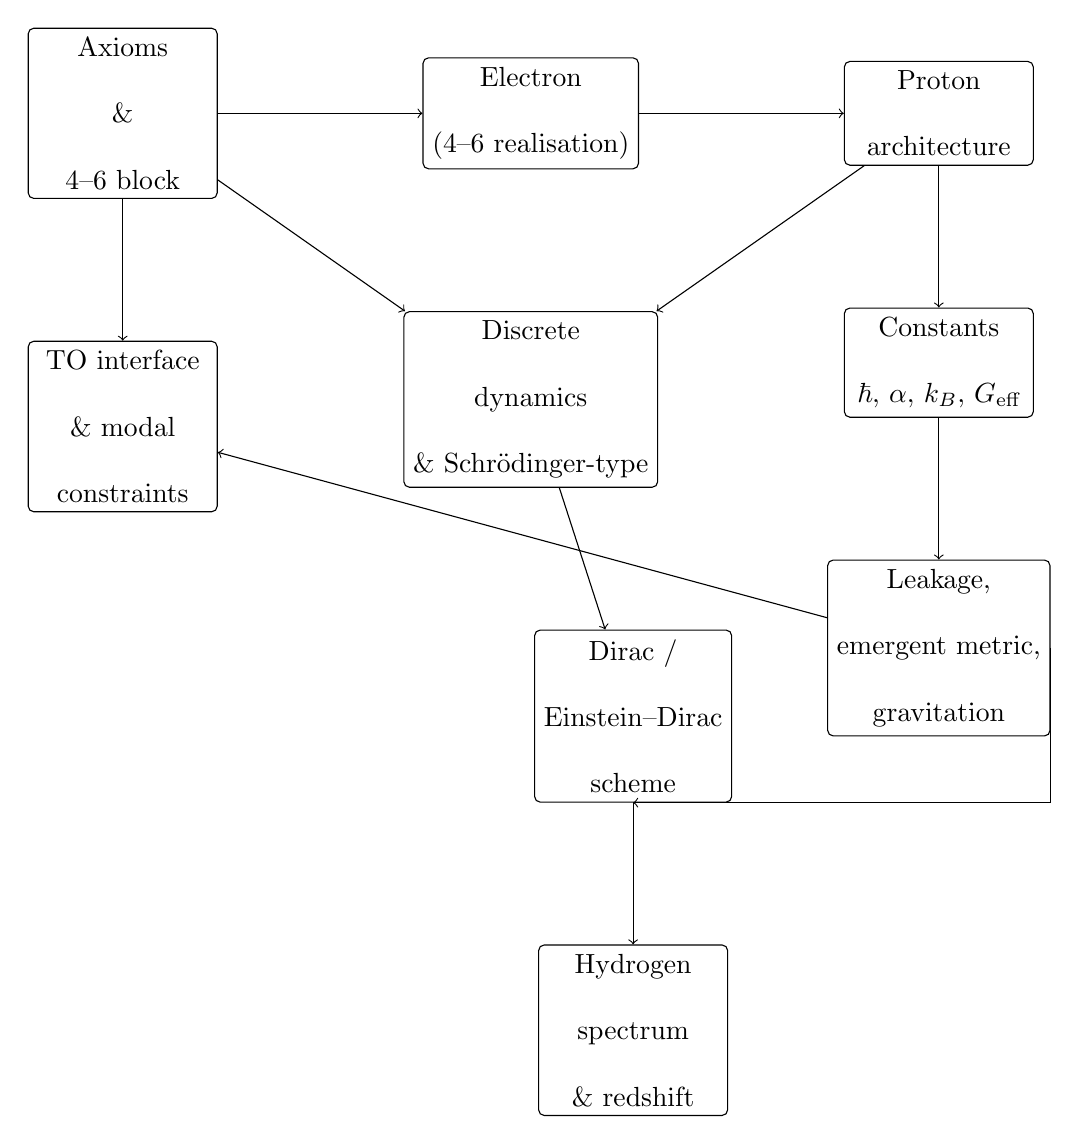
\begin{tikzpicture}[
    node distance=1.6cm,
    box/.style={draw, rectangle, rounded corners=2pt, align=center, minimum width=2.4cm, minimum height=0.9cm}
  ]
    % Ligne du haut
    \node[box] (axioms) {Axioms \\\\ \&\\\\ $4$--$6$ block};
    \node[box, right=2.6cm of axioms] (electron) {Electron \\\\ ($4$--$6$ realisation)};
    \node[box, right=2.6cm of electron] (proton) {Proton \\\\ architecture};

    % Colonne centrale droite : constantes, métrique
    \node[box, below=1.8cm of proton] (constants) {Constants \\\\ $\hbar,\, \alpha,\, k_B,\, G_{\text{eff}}$};
    \node[box, below=1.8cm of constants] (metric) {Leakage, \\\\ emergent metric, \\\\ gravitation};

    % Colonne centrale gauche : dynamique
    \node[box, below=1.8cm of electron] (dynamics) {Discrete \\\\ dynamics \\\\ \& Schr\"odinger-type};

    % Nouveau nœud : Dirac / Einstein–Dirac
    \node[box, below=1.8cm of dynamics, xshift=1.3cm] (einsteindirac) {Dirac / \\\\ Einstein--Dirac \\\\ scheme};

    % Nœud de test phénoménologique (optionnel mais clair)
    \node[box, below=1.8cm of einsteindirac] (hydrogen) {Hydrogen \\\\ spectrum \\\\ \& redshift};

    % Colonne gauche : interface TO
    \node[box, below=1.8cm of axioms] (TO) {TO interface \\\\ \& modal \\\\ constraints};

    % Flèches existantes
    \draw[->] (axioms) -- (electron);
    \draw[->] (electron) -- (proton);
    \draw[->] (proton) -- (constants);
    \draw[->] (constants) -- (metric);
    \draw[->] (axioms) -- (dynamics);
    \draw[->] (proton) -- (dynamics);
    \draw[->] (axioms) -- (TO);
    \draw[->] (metric) -- (TO);

    % Nouvelles flèches pour le bloc Einstein–Dirac
    \draw[->] (dynamics) -- (einsteindirac);
    \draw[->] (metric.east) |- (einsteindirac.south); % métrique -> Einstein–Dirac (par la droite)
    \draw[->] (einsteindirac) -- (hydrogen);

  \end{tikzpicture}
  \caption{Schematic dependency structure within the PDL programme, including the Dirac / Einstein--Dirac scheme.}
  \label{fig:pdl_dependency}
\end{figure}


\subsection{Classification scheme}
\label{subsec:classification_scheme}

To monitor the internal coherence of the PDL programme and to render its susceptibility to revision explicit, we assign each principal component to one of three epistemic categories:
\begin{itemize}[leftmargin=1.5em]
  \item \textbf{Proven structural result:} a statement that is derived exclusively from the axioms and combinatorial analysis, without recourse to phenomenological input.
  \item \textbf{Tightly constrained conjecture:} a statement that depends on additional, explicitly formulated modelling assumptions, but is nevertheless strongly restricted by the axioms, internal consistency requirements, and multiple quantitative correspondences.
  \item \textbf{Empirically calibrated element:} a statement or construct that depends on at least one parameter whose numerical value is determined by fitting to experimental data, and which has not yet been rigorously derived from the axioms.
\end{itemize}

\subsection{Summary tables}
\label{subsec:summary_tables}

Table~\ref{tab:status} provides an overview of the current epistemic status of selected core components of the PDL framework. This catalogue will be progressively expanded as the programme advances and further developments are integrated.

\setlength{\LTpre}{18pt}
\setlength{\LTpost}{0pt}

\begin{longtable}{@{}p{0.7cm}p{7cm}L{5.6cm}p{2cm}@{}}
  \caption{Preliminary global map of key PDL items and their epistemic status.}
  \label{tab:status}\\

  \toprule
  ID & Item & Status & Main sources \\
  \midrule
  \endfirsthead

  \toprule
  ID & Item & Status & Main sources \\
  \midrule
  \endhead

  \bottomrule
  \endfoot

  L1 &
  Relational axioms (binary pulsation, triangular coherence, minimal completeness, logical optimisation) and demonstration of the existence of the minimal 4–6 block as the first admissible elementary stationary closure &
  Established structural theorem & \cite{PDL_Main_2026,PDL_intro,PDL_position} \\[0.4em]

  L2 &
  Interpretation of the 4–6 logical stationary regime as a prototypical representation of an electron at rest (with Compton pulsation modeled as an internal two-cycle and $\hbar$ identified as the minimal action per coherence cycle) &
  Stringently constrained conjecture &
  \cite{PDL_Main_2026,PDL_intro} \\[0.4em]

  P1 &  
  Hierarchical proton architecture characterized by the integer invariants (24, 28, 930, 10087, 11017) and a stationary-to-dynamical partition of approximately $\sim 9\%/91\%$ &  
  Formulation of a tightly constrained conjecture & \cite{PDL_Main_2026,Combinatorial_Proton_v2_2026,PDL_intro,PDL_position} \\[0.4em]

  C1 &
  Reinterpretation of $\hbar$ as the minimal coherence expenditure associated with a single internal cycle within the 4--6 regime &
  Stringently constrained conjecture &
  \cite{PDL_Main_2026,PDL_intro} \\[0.4em]

  C2 &
  Closed-form expression for the inverse fine-structure constant, $\alpha^{-1}$, formulated in terms of the proton–electron mass ratio, the valence content $r_{\mathrm{val}} = 930$, and the golden ratio, which reproduces the empirical value with a relative accuracy of $\mathcal{O}(10^{-4})$ without recourse to continuously tunable fitting parameters. &
  Stringently constrained conjecture (quantitatively successful) & \cite{Alpha_PDL_v2_2026,PDL_intro,Born_Golden_v2_2026} \\[0.4em]

  C3 &
  Candidate expression for the Boltzmann constant $k_B$, formulated in terms of the same discrete architectural framework, the electron’s minimal pulsation, the dynamical fraction of the proton sea, and a single leakage parameter $\varepsilon$ &
  Stringently constrained conjecture with partial empirical calibration & \cite{PDL_Main_2026,PDL_position,Coherence_Leakage_18_2026} \\[0.4em]

  BR1 & 
  Relational emergence and a Gleason-type uniqueness theorem for Born’s rule are derived for spin-$\tfrac{1}{2}$ measurement processes within the formal framework of Propositional Dynamic Logic (PDL). The analysis proceeds via a mixed-triangle scheme that satisfies a comprehensive set of operational axioms, including normalization, phase invariance, rotational covariance, and measurement repeatability, thereby providing a mathematically rigorous and operationally well-grounded characterization of the underlying probabilistic structure. & 
  Previously established structural theorem, applicable under the stipulated symmetry conditions and operational assumptions & \cite{Gleason_PDL_2026,Golden_Ratio_Sketch_2026} \\[0.4em] 
  
  EF1 & 
  Discrete analogues of Gauss’s and Faraday’s laws are formulated in terms of mixed-triangle coherence fluxes defined on signed graphs. These discrete constructions reproduce Coulomb-like $1/r^{2}$ field profiles via shell-counting procedures and yield simplified (toy) models of emergent Schrödinger dynamics that are compatible with the Planck–de Broglie–Lorentz (PDL)-based expression for the fine-structure constant $\alpha$. &
  Stringently delimited conjecture (structurally well-defined, with its dynamical components presently subject to ongoing refinement) &  \cite{Effective_Fields_PDL_2026,Coherence_Leakage_18_2026} \\[0.4em]

  G1 &
 Effective gravitational coupling emerging from nucleonic coherence–leakage mechanisms, formulated as a function of the fundamental constants $\hbar$, $c$, $m_p$, the fine-structure constant $\alpha$, and a leakage parameter $\varepsilon$, the latter entering the expression as a highly amplified contribution raised to the 18th power. &
  Empirically constrained parameter (functional dependence fixed; $\varepsilon$ calibrated such that the observed value of $G$ is reproduced) & \cite{PDL_Main_2026,Exponent_18_PDL_2026,PDL_position} \\[0.4em]

  D1 &  
  The rigorously established existence of discrete, graph-theoretic evolutionary frameworks that accurately reproduce Schrödinger-type dynamics—specifically, dynamics governed by Laplacian operators and subject to flux-balance (continuity) constraints—in suitably defined coarse-grained continuum limits. &  
  An active research area in dynamical systems theory with strong theoretical support, though a fully rigorous general proof is still lacking. & \cite{Coherence_Leakage_18_2026,Schrodinger_Sketch_v2_2026,PDL_position} \\[0.4em]

  ED1 & 
  Exploratory Einstein--Dirac extension of the PDL framework, in which Dirac spinor degrees of freedom are associated with $(4,6)$ electron closures and coupled to an emergent metric derived from coherence costs; includes preliminary consistency checks based on hydrogen-like spectra, redshift scenarios, and the recovery of appropriate Schr\"odinger-type limits. & 
  Early-stage conjectural framework (conceptually motivated, technically under active development) & \cite{Einstein_Dirac_PDL_2026,PDL_Main_2026,Coherence_Leakage_18_2026,Coherence_Leakage_18_2026} \\[0.4em]

  M1 &
  Coexistence topology, a coherence-cost pseudometric defined on closure spaces, and the interpretation of logical leakage as a self-maintaining probability distribution associated with quantum statistical structures and emergent gravitational dynamics &
  Strongly constrained conjecture & \cite{Coherence_Leakage_18_2026,PDL_position} \\[0.4em]

  COS1 & 
  Cosmological framework derived from constraint-based events in a pre-physical logical domain: generation and recycling of closure structures, interpretation of the cosmological constant as a manifestation of residual coherence, and emergence of large-scale structure as an organized pattern of relational density. & 
  Speculative conceptual elaboration (extending beyond the scope of the core empirically testable claims) & \cite{PDL_Main_2026,PDL_position} \\[0.4em]

  TO1 &
  Informal mappings between structures in Propositional Dynamic Logic (PDL) and the absolute truths A1–A7 postulated in the Theory of Objectivity (TO)—namely: nothingness, aura, boundaries, multi-observer stabilisation, and transcendent substrate. &
  Conceptual framework currently under development & \cite{PDL_TO_dialogue,PDL_position} \\

\end{longtable}

\subsection{Dependency diagram (conceptual)}

\begin{figure}[H]
  \centering
  % Simple placeholder; can be replaced with a real TikZ diagram later
  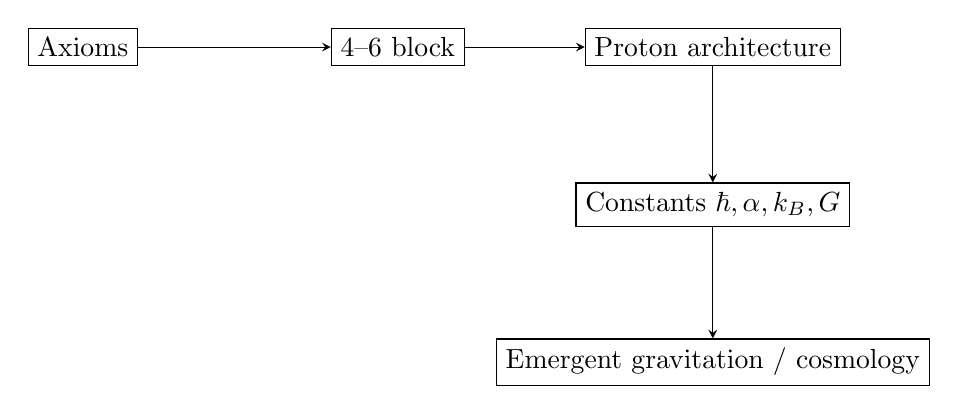
\begin{tikzpicture}[node distance=2cm,>=stealth,->]
    \node (axioms) [draw, rectangle] {Axioms};
    \node (fourSix) [draw, rectangle, right of=axioms, xshift=2cm] {4--6 block};
    \node (proton) [draw, rectangle, right of=fourSix, xshift=2cm] {Proton architecture};
    \node (constants) [draw, rectangle, below of=proton] {Constants \(\hbar,\alpha,k_B,G\)};
    \node (grav) [draw, rectangle, below of=constants] {Emergent gravitation / cosmology};

    \draw (axioms) -- (fourSix);
    \draw (fourSix) -- (proton);
    \draw (proton) -- (constants);
    \draw (constants) -- (grav);
  \end{tikzpicture}
  \caption{Schematic dependency chain within PDL.}
  \label{fig:dependency}
\end{figure}

\section{Roadmap and Future Work}
\label{sec:roadmap}

\subsection{Foundational and combinatorial tasks}
\label{subsec:roadmap_foundational}

Several foundational combinatorial problems are central to the further development of the PDL programme. A first priority is the uniqueness question for the minimal $4$–$6$ block: obtaining a rigorous proof or disproof that no smaller or alternative configuration satisfies the axioms with comparable optimality would determine whether the $4$–$6$ regime is a strictly necessary primitive or merely one admissible choice among a broader class of structures \cite{PDL_Main_2026,PDL_position}. A second major objective is the exhaustive classification of admissible proton architectures in a neighbourhood of the integer tuple $(24,28,930,10087,11017)$, with the aim of establishing whether the currently preferred proton model is uniquely determined (up to isomorphism) by the optimisation constraints, or whether a nontrivial family of degenerate alternatives is admitted \cite{Combinatorial_Proton_v2_2026,PDL_position}. A third foundational goal is a fully combinatorial derivation of the leakage parameter $\varepsilon$ and the exponent $18$ from intrinsic graph-theoretic invariants of hierarchical closures, thereby eliminating the present dependence on calibration against the empirical value of $G$ and promoting gravitation from a partially fitted effect to a fully predicted emergent coupling \cite{Exponent_18_PDL_2026,Coherence_Leakage_18_2026,PDL_position}.

\subsection{Dynamical and phenomenological extensions}
\label{subsec:roadmap_dynamical}

On the dynamical side, a central objective is to specify and rigorously analyse a canonical class of graph-evolution rules that satisfy the PDL axioms, implement energy as a coherence cost, and reproduce Schr\"odinger-type evolution equations in suitable coarse-grained limits \cite{Coherence_Leakage_18_2026,Coherence_Leakage_18_2026}. This entails elucidating the mechanisms by which probability amplitudes, interference patterns, and measurement-like phenomena emerge from discrete coherence flows on signed graphs. At the phenomenological level, the current benchmarks based on the hydrogen atom must be generalised to more complex systems, including other nuclei, hydrogen-like ions, simple multi-electron atoms, and condensed-matter configurations \cite{PDL_Main_2026,Schrodinger_Sketch_v2_2026}. Such generalisations will enable a systematic investigation of the scaling behaviour of coherence-ratio descriptions and provide a stringent test of whether the PDL architecture remains self-consistent as structural and dynamical complexity increase \cite{PDL_position}.

\subsection{Interface and comparison with other frameworks}
\label{subsec:roadmap_interface}

A further strand of research is devoted to the systematic comparison of PDL with other foundational frameworks. This programme includes confronting the discrete coherence structures of PDL with quantum field theory and quantum chromodynamics—particularly in relation to proton structure and mass decomposition—as well as with quantum information–theoretic reconstructions of quantum theory, and with discrete or holographic approaches such as causal set theory, loop-based models, and tensor network formalisms \cite{PDL_intro,PDL_position}. The overarching objective is to delineate the regimes in which PDL reproduces established results, yields genuinely novel insights, or can be subjected to decisive empirical or theoretical falsification. In parallel, an intensified engagement with the Theory of Objectivity and related modal–axiomatic programmes is expected to refine the ontological interpretation of PDL, particularly with regard to boundaries, multi-observer stabilisation, and the status of the leakage parameter as a candidate for a transcendent substrate \cite{PDL_TO_dialogue,PDL_position}.

\subsection{Planned updates of this mapping document}
\label{subsec:roadmap_mapping}

This mapping document is conceived as a dynamic, continuously updated overview of the PDL programme. It will be revised whenever major milestones are achieved, such as the establishment of a uniqueness theorem for the $4$--$6$ block, a combinatorial derivation of $\varepsilon$, a mathematically robust account of emergent Schr\"odinger dynamics, or substantial modifications of the proton architecture \cite{PDL_position}. Subsequent revisions will refine the global result map, introduce or amend entries in the document index, and adjust the dependency diagrams to accurately represent the evolving internal structure of the programme. Negative results and counterexamples will be documented explicitly, ensuring that the mapping continues to serve as a transparent structural framework for evaluating both the advances and the limitations of the PDL approach \cite{PDL_position}.

\newpage

\appendix

\section{Document Index and Cross-References}
\label{app:doc_index}

Table~\ref{tab:doc_index} summarises the principal PDL documents, the internal identifiers employed for them in this mapping (D1, D2, \dots), and a concise description of the sections of the present work in which each document is predominantly utilised.

\setlength{\LTpre}{18pt}
\setlength{\LTpost}{0pt}

\begin{longtable}{@{}p{0.9cm}L{5cm}L{5cm}p{4.4cm}@{}}
  \caption{Index of PDL documents and their role in this mapping.}
  \label{tab:doc_index}\\

  \toprule
  Label & Document & Main thematic domain & Sections of this mapping \\
  \midrule
  \endfirsthead

  \toprule
  Label & Document & Main thematic domain & Sections of this mapping \\
  \midrule
  \endhead

  \bottomrule
  \endfoot

  D1 &
  The Emergence of Physical Reality within the Framework of the Projective Dynamic Logo (PDL) &
  Core axioms, $4$--$6$ block, proton architecture, constants, gravitation, cosmology &
  \ref{sec:logical_core}, \ref{sec:four_six_electron}, \ref{sec:proton_architecture}, \ref{sec:constants}, \ref{sec:topology_metric} \\[0.4em]

  D2 &
  Introduction to the Projective Dynamic Logo (PDL) &
  High-level conceptual overview and summary of key structures and constants &
  \ref{sec:overview}, \ref{subsec:core_question}, \ref{sec:constants}, \ref{sec:roadmap} \\[0.4em]

  D3 &
  Projective Dynamic Logo as a Foundational Research Programme (Position Paper) &
  Status, epistemic classification, open problems, TO dialogue, global mapping of results &
  \ref{sec:overview}, \ref{sec:global_map}, \ref{sec:TO_interface}, \ref{sec:roadmap} \\[0.4em]

  D4 &
  On the Combinatorial Selection of the Proton Architecture in PDL (v2) &
  Detailed proton integers, optimisation constraints, alternative candidates, updated selection functional &
  \ref{sec:proton_architecture}, \ref{subsec:roadmap_foundational} \\[0.4em]

  D5 &
  A Structural Derivation of the Fine-Structure Constant from the Projective Dynamic Logo (PDL) (v2) &
  Derivation and numerical assessment of the PDL expression for $\alpha$, including post-TO refinements &
  \ref{sec:constants}, \ref{subsec:constants_table}, \ref{sec:global_map} \\[0.4em]

  D6 &
  Relational Emergence of Born's Rule and a Golden-Ratio Active Surface in PDL (v2) &
  Born's rule for spin-$\tfrac{1}{2}$, golden-ratio active surface, refined link between surface partition and $\alpha$ &
  \ref{sec:logical_core}, \ref{sec:constants}, \ref{sec:global_map} \\[0.4em]

  D7 &
  From Discrete Coherence Flux to Effective Fields: A Structured Programme within the PDL Framework &
  Discrete Gauss–Faraday structure, effective fields, Coulomb profiles, link to Schr\"odinger-type dynamics &
  \ref{sec:dynamics}, \ref{sec:topology_metric}, \ref{sec:global_map} \\[0.4em]

  D8 &
  A Minimal Relational Sketch for the Emergence of the Golden Ratio in PDL &
  Core–surface partition of the proton, emergence of the golden ratio, constraints on active surface &
  \ref{sec:proton_architecture}, \ref{sec:constants} \\[0.4em]

  D9 &
  Hierarchical Filtering of Coherence Leakage and Justification of the Exponent 18 in PDL &
  Original formulation of leakage filters and exponent $18$ as total number of hierarchical filters &
  \ref{sec:topology_metric}, \ref{subsec:roadmap_foundational} \\[0.4em]

  D10 &
  Logical Leakage as Self-Maintained Probability: A Topological Reformulation in the Projective Dynamic Logo Framework &
  Coexistence topology, coherence-cost pseudo-metric, probabilistic reinterpretation of leakage &
  \ref{sec:topology_metric}, \ref{sec:dynamics}, \ref{sec:global_map} \\[0.4em]

  D11 &
  Compatibility of the Schr\"odinger Framework with the Projective Dynamic Logo (PDL) (v2) &
  Effective insertion of PDL-derived $\alpha$ and proton structure into hydrogenic Schr\"odinger equation, updated numerical checks &
  \ref{sec:dynamics}, \ref{sec:global_map} \\[0.4em]

  D12 &
  Towards a Schr\"odinger--Type Dynamics from the Projective Dynamic Logo (PDL): A Relational Sketch Linking Coherence Cycles, Active Surfaces, and Effective Potentials (v2) &
  Toy models and preliminary derivations of Schr\"odinger-like dynamics from graph evolution, refined consistency conditions &
  \ref{sec:dynamics}, \ref{subsec:roadmap_dynamical} \\[0.4em]

  D13 &
  A Modal Dialogue between the Projective Dynamic Logo (PDL) and the Theory of Objectivity (TO) &
  Comparison with TO's Absolute Truths, boundary and multi-observer issues, transcendent substrate &
  \ref{sec:TO_interface}, \ref{subsec:roadmap_interface} \\[0.4em]

  D14 &
  Towards an Einstein--Dirac Unification from the Projective Dynamic Logo Framework &
  Einstein–Dirac extension, Dirac spinors on $(4,6)$ closures, coupling to emergent metric, preliminary consistency checks &
  \ref{sec:dynamics}, \ref{sec:topology_metric}, \ref{subsec:roadmap_dynamical} \\[0.4em]

  D15 &
  Minimal Stationary Closures in the Projective Dynamic Logo Framework: Necessity of the (4,6) Block &
  Detailed analysis of minimal stationary closures, non-existence for $n \leq 3$, necessity and quasi-uniqueness of the $(4,6)$ block &
  \ref{sec:logical_core}, \ref{subsec:4_6_block}, \ref{sec:global_map} \\[0.4em]

  D16 &
  On the Combinatorial Selection and Local Uniqueness of the Proton Architecture in the PDL Framework &
  Refined combinatorial analysis of proton configurations, definition of selection functional, local uniqueness conjecture &
  \ref{sec:proton_architecture}, \ref{subsec:roadmap_foundational} \\[0.4em]

  D17 &
  Coherence Leakage, Hierarchical Filtering, and the Exponent 18 in the Projective Dynamic Logo Framework &
  Refined treatment of coherence leakage, intrinsic $\varepsilon$ on proton graphs, organisation of 18 filters, effective coupling ansatz for $G_{\mathrm{eff}}^{\PDL}$ &
  \ref{sec:topology_metric}, \ref{sec:global_map}, \ref{subsec:roadmap_foundational} \\[0.4em]

\end{longtable}

\newpage

\section{Glossary of Selected Terms}
\label{app:glossary}

\begin{description}[style=nextline,leftmargin=1.5cm]
  \item[Closure] A finite signed graph that realises a self-sustaining regime of
  coherence under the PDL axioms, exhibiting minimal or otherwise controlled
  leakage.

  \item[Logical stationary regime] A configuration whose internal sign
  pattern sustains a non-trivial cyclic evolution (typically a 2-cycle)
  that preserves triangular coherence and does not rely on external input.

  \item[Coherence cost] A quantitative measure of the relational “effort”
  necessary to maintain a given closure; in physical instantiations, this
  quantity can be identified with energy via relations such as \(E = \hbar \omega\).

  \item[Active surface] The subset of relations within a composite structure
  (for example, the proton) that actually participate in coherent coupling to
  external closures, in contrast to relations that are dedicated exclusively
  to internal stabilisation.

  \item[Leakage] The minimal, irreducible defect of closure in hierarchical
  structures, parameterised by \(\varepsilon\); this is interpreted both as
  a source of effective probabilistic behaviour and as the origin of emergent
  gravitational coupling.

  \item[Coexistence topology] The topology on the space of closures induced by
  their mutual compatibility; two closures are considered “close” if they can
  be jointly embedded with a low additional coherence cost.

  \item[Coherence-cost pseudo-metric] A distance-like function on the space of
  closures, which measures the extra coherence expenditure required to render
  them coexistent within a common environment; this provides the discrete
  substrate for an emergent metric structure.

\end{description}

\newpage

\section{Glossary of Key Terms}
% Closure, coherence budget, leakage, active surface, etc.

\bibliographystyle{unsrturl}
\bibliography{references}

\end{document}
